\section{Wstęp: }
\subsection{Algorytm Genetyczny}
  Algorytmy genetyczne są heurystykami, które działają w oparciu o przeszukiwanie
  przestrzeni rozwiązań w celu wyszukania najlepszego rozwiązania względem
  zadanego krytermium. Nazwa ów algorytmu pochodzi od sposobu działania, który
  przypomina znane w przyrodzie zjawisko ewolucji biologicznej. \\
  Algorytm genetyczny rozpoczyna pracę poprzez wybranie pewnej grupy osobników,
  którą będziemy nazywać \textbf{populacją}. Każda osobnik należący do populacji
  posiada przypisane pewne informacje, które stanowią jego \textbf{genotyp}, na podstawie
  którego tworzony jest \textbf{fenotyp}. Genotyp opisuje proponowane rozwiązanie problemu, a fenotyp przedstawia nam, jak dobre jest to rozwiązanie 
  (tu: funkcja celu). Genotyp składa się z \textbf{chromosomów}, natomiast chromosomy składają
  się z \textbf{genów}. W naszym przypadku pojedynczym genem będzie jedno miasto. 
  Po wygenerowaniu populacji początkowej algorytm dokonuje szeregu operacji, których zadaniem
  jest przystowanie osobników do danego środowiska. W naszym przypadku algorytm
  będzie dążył do redukcji funkcji celu. \\
  Przed rozpoczeciem działania algorytm pobiera od użytkownika szereg informacji,
  które w znaczy sposób mogą wpłynąć na wydajność jak i ostateczny wynik
  wyprodukowany przez algorytm. Parametry zależne od użytkownika to:
  \begin{itemize}
    \item Maksymalna liczba iteracji algorytmu (jest to również warunek końcowy działania programu) reprezentowany przez nieujemną liczbą całkowitą
    \item Współczynnik mutacji- liczba wymierną z zakresu $[0,1]$, która przedstawia z jaką szansą dany osobnik może ulec mutacji
    \item Współczynnik selekcji- W zależności od trybu działania programu parametr przyjmuje jedną z dwóch form:
    \begin{itemize}
      \item Nieujemną liczbę całkowitą w przypadku skorzystania z turnieju. Wtedy ów liczba reprezentuje z ilu uczestników turnieju wybieramy rodziców do dalszego krzyżowania
      \item Liczbę wymierną z zakresu $[0,1]$, która przedstawia jaki procent populacji ulegnie krzyżowaniu. Wybierając liczbę 0.7 przypisujemy operacji krzyżowania $70\%$ najlepszych osobników, $30\%$ najgorszych nie ulegnie ewolucji i zostanie zastąpiona (odcięcie)
      \item Liczbę wymierną z zakresu $[0,1]$, która wykorzysytywana jest w metodzie selekcji typu ruletka, która polega na znomrmalizowaniu współczynnika dopasowania tak, że suma wszystkich wynosi 1 odwrotnie propocjonalnie do długości ścieżki.
    \end{itemize}
    \item Rozmiar populacji określający ilu osobników wchodzi w skład populacji
    \item Maksymalna liczba iteracji bez poprawy, której przekroczenie uruchamia specjalną procedurę mającą na celu rozwiązanie problemu stagnacji oraz potencjalnej zbieżności osobników
    \item Maksymalny wiek- jeśli osobnik osiągnie maksymalny wiek zostanie poddany specjalnej procedurze modyfikującej oraz jego wiek zostanie zresetowany. Ma to na celu zapobieganie stagnacji oraz zbyt szybkiej zbieżności osobników do najstarszego, najlepiej przystosowanego
  \end{itemize}
  W trakcie swojego działania algorytm wykonuje następujące kroki:
  \begin{enumerate}
    \item Pierwszym krokiem jest wygenerowanie pierwszej populacji przy użyciu metody \textbf{generate population()}
    \item Dochodzi do operacji selekcji osobników, która realizowana jest przez metodę \textbf{selection()}. 
    W zależności od wyboru użytkownika, selekcja jest przeprowadzana w formie turnieju lub ogranieczenia zbioru populacji do wskazanego procenta, najsłabi osobnicy poza wskazanym procentem są nadpisywani przez najlepszych (tak zwane \textbf{Odcięcie}).
    \item Przy użyciu metody \textbf{crossover()} dochodzi do operacji krzyżowania, która wykorzystując dwóch osobników z obecnej populacji (tak zwanych \textbf{rodziców}) generuje nowych dwóch osobników (\textbf{dzieci}).
    Generowanie dzieci zachodzi poprzez wymianę genów między rodzicami z zachowaniem własności cyklu Hamiltona. Z reguły generacja drugiego dziecka przebiega identycznie do wygenerowania drugiego,
    z jedyną różnicą zamiany kolejności rodziców w argumentach wywowałnia funkcji. Wykorzystane metody krzyżowania to:
    \begin{enumerate}
      \item Partially Mapped Crossover (PMX)
      \item Order Crossover (OX)
      \item Half Crossover (HX)
    \end{enumerate}
    \item Metoda \textbf{mutation()} odpowiada za dokonywanie mutacji osobników populacji ze wskazanym przez użytkownika prawdopodobieństwem.
    W celu dokonywania mutacji zaimplementowano dwie metody
    \begin{enumerate}
      \item Znana metoda z algorytmu two opt - invert, która dokonuje inwersji kawałka drogi między dwoma losowo wybranymi miastami
      \item RGIBNNM - metoda, która poza invertem wyszukuje najbliższego sąsiada losowego miasta i dokonuje z nim operacji zamiany miejscami. Ów metoda dodatkowo jest
      wykorzystywana w celu uniknięcia procesu stagnacji
    \end{enumerate}
    \item Dla każdego osobnika z populacji zostaje dodany wiek. Osobnicy przekraczający maksymalny wiek zostają poddani procesowi "odmłodzenia" przy pomocy metody \textbf{unstack()}
    \item Po wygenerowaniu nowej populacji znajdujemy najbardziej przystosowanego do warunków zadania osobnika. Jeśli jest on lepszy, niż obecnie znaleziony osobnik
    to dokonujemy nadpisania i przechodzimy do następnego etapu
    \item Opcjonalny etap, który polega na wykonaniu operacji \textbf{unstack()} w sytuacji, gdy algorytm wykryje wystąpenie stagnacji
  \end{enumerate}
  \textbf{UWAGA}: Kroki 2-7 wykonywane są w pętli, której warunkiem końcowym jest liczba iteracji podana przez użytkownika jako jeden z argumentów uruchomienia programu. \\
 \textbf{Złożoność obliczeniowa: }
    Główna pętla programu znajduje się w metodzie o nazwie \textbf{populate()}. Analiza złożoności obliczeniowej zostanie wykonana poprzez analizę poszczególnych metod
    wykonywanych w trakcie działania głównej pętli. Przyjmujemy, że liczba wykonań pętli \textbf{while()} jest wartością stałą.
    \begin{enumerate}
      \item \textbf{Generate Population} - W tej metodzie dochodzi do wygenerowania początkowej populacji. Ze względu na fakt, iż uzyskae wyniki zależą od początkowej populacji 
      w realizacji programu zdecydowaliśmy się na dwie metody generowania populacji. Drugą z nich jest \textbf{Improve Atsp}, której omówienie znajduje się poniżej.
      W ów metodzie generujemy liczbę osobników równą rozmiarowi populacji. Rozmiar populacji jest liczbą stałą podaną przez użytkownika.
      W pętli głównej dochodzi do wygenerowania osobników dwoma sposobami. Jednym z nich jest wykonanie funkcji \textbf{shuffle()}, drugą jest wykorzystanie
      wcześniej zaimplementowanego algorytmu \textbf{K random()} ze stałą równą \textit{10}. 
      Złożoności obliczeniowa ów metod generujących to odpowiednio: \textbf{$O(n)$} oraz \textbf{$O(n$)}. Reasumując dochodzimy do wniosku, iż złożoność obliczeniowa
      rozpatrywanej metody wynosi \textbf{$O(k*n)$}, gdzie $k$ oznacza rozmiar populacji.
      \item \textbf{Improve atsp} - W tej metodzie dodatkowo generujemy 5 osobników korzystając z metody najbliższego sąsiada, której implementacją oraz analizą zajmowaliśmy się w ramach pierwszej listy zadań, stąd wiemy 
      iż jej złożoność obliczeniowa jest równa $O(n^2*log n)$. Dodatkowo do lekkiego wymieszania osobników wykorzystujemy metodę \textbf{unstack()}, której złożoność wynosi \textbf{$O(k*n)$}, gdzie $k$ to rozmiar populacji (co zostanie wykazane w późniejszej częście sprawozdania).
      \item \textbf{Find Best} - Metoda znajdująca najlepszego osobnika po funkcji celu wykorzystująca wbudowaną w pythonie funkcję \textbf{min()}. Złożoność obliczeniowa- \textbf{$O(n)$}.
      \item \textbf{Selection} - Metoda dokonująca selekcji osobników. W zależności od użytej metody otrzymujemy różne złożoności obliczeniowe:
      \begin{itemize}
        \item Wykorzystując odcięcie jedyną problematyczną z punktu widzenia złożoności operacją jest operacja sortowania, która przy wykorzystaniu wbudowanej metody \textbf{sorted()} wykonuje się w czasie \textbf{$O(n*log n)$},
        \item Wykorzystując turniej losujemy z populacji daną część osobników, z której następienie wybieramy dwóch najlepszych. Jak powyżej, ze względu na wykonanie sortowania otrzymujemy złożonosć równą \textbf{$O(k*n*log n)$}, gdzie $k$ jest rozmiarem populacji a $n$ liczbą wybieranych osobników
        \item Korzystając z ruletki 
      \end{itemize}
      \item \textbf{Crossover} - Metoda dokonująca krzyżowań, która wykonuje się w czasie liniowym względem liczności populacji
      \item \textbf{Mutation} - Metoda dokonująca mutacji, która wykonuje się w czasie liniowym względem liczności populacji
      \item \textbf{Add Age} - Metoda dodająca wiek do każdego członka populacji wykonująca się w czasie liniowym względem liczby populacji 
      \item \textbf{Unstack} - Metoda wykorzystywana do uniknięcia stagnacji oraz przedwczesnych zbieżności, która wykonuje się w czasie liniowym względem liczby populacji 

    \end{enumerate}
  \textbf{Wykresy:}
  Na poniższych wykresach eksperymentalnie wykazaliśmy przedstawioną powyżej złożoność obliczeniową. 
  Do testów wykorzystaliśmy instancje \textbf{berlin52} oraz \textbf{gr24}, które znajdują się w bibliotece TSPLIB.
  Dodatkowo badanymi parametrami były liczba iteracji oraz rozmiar populacji.
  \begin{figure}[H]
    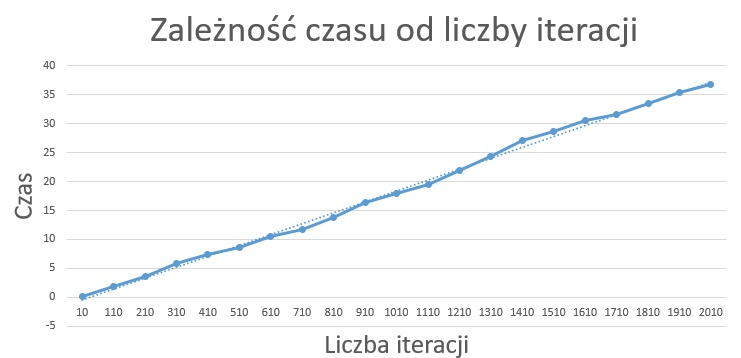
\includegraphics[scale=0.75]{berlin52Iter.png}
    \centering
    \caption{Zależność czasu od liczby iteracji dla instancji berlin52}
  \end{figure}
  \begin{figure}[H]
    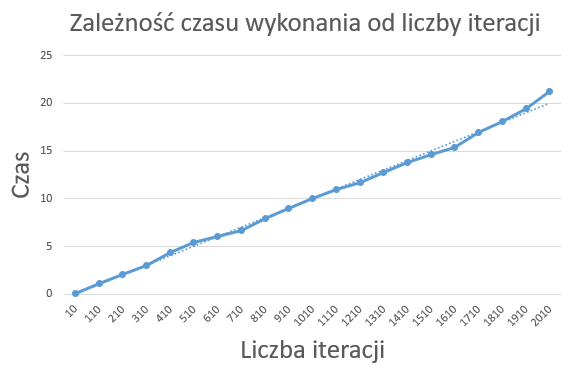
\includegraphics[scale=0.75]{gr24Iter.png}
    \centering
    \caption{Zależność czasu od liczby iteracji dla instancji gr24}
  \end{figure}
  \begin{figure}[H]
    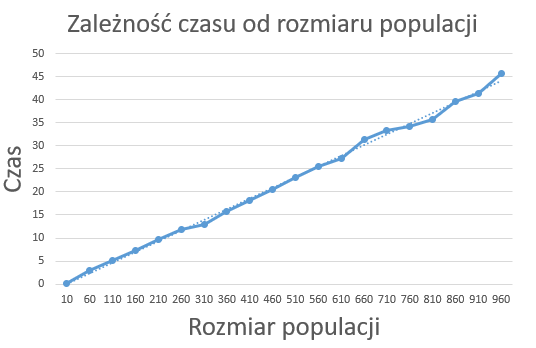
\includegraphics[scale=0.75]{berlin52Pop.png}
    \centering
    \caption{Zależność czasu od rozmiaru populacji dla instancji berlin52}
  \end{figure}
  \begin{figure}[H]
    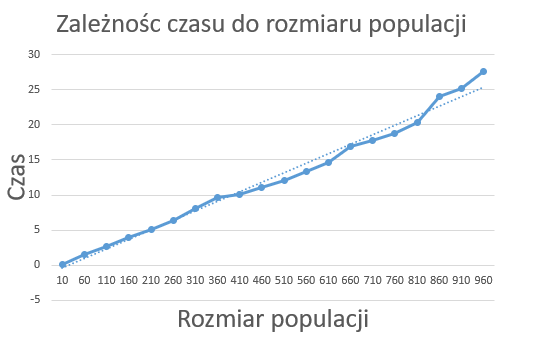
\includegraphics[scale=0.75]{gr24Pop.png}
    \centering
    \caption{Zależność czasu od rozmiaru populacji dla instancji gr24}
  \end{figure}

  \textbf{Wniosek:} Złożoność obliczeniowa metody \textbf{populate()} wynosi \textbf{$O(k*n*log n)$}, gdzie k oznacza liczbę iteracji, a n- rozmiar populacji. \\
  Przyglądając się otrzymanym wykresom zauważamy, iż przypominają one bardziej linię prostą aniżeli $n*logn$. Zapewne wynika to z faktu, iż rozmiar populacji jest zdecydowanie mniejszy niż rozmiar populacji.\\
 \textbf{Złożoność pamięciowa: }
